\section{Ejercicio 4}

Este ejercicio propone realizar lo mismo que el ejercicio anterior pero en vez de usar MSE para calcular la pérdida se utilzó CCE (\textit{Categorical Cross Entropy}).

El grafo computacional es el mismo que el obtenido para el ejercicio 3, con la salvedad que la función de costo (último bloque del grafo) es la función CCE.

El resultado obtenido para este problema es:

\begin{figure}[H]
     \centering
     \begin{subfigure}[b]{0.45\textwidth}
         \centering
         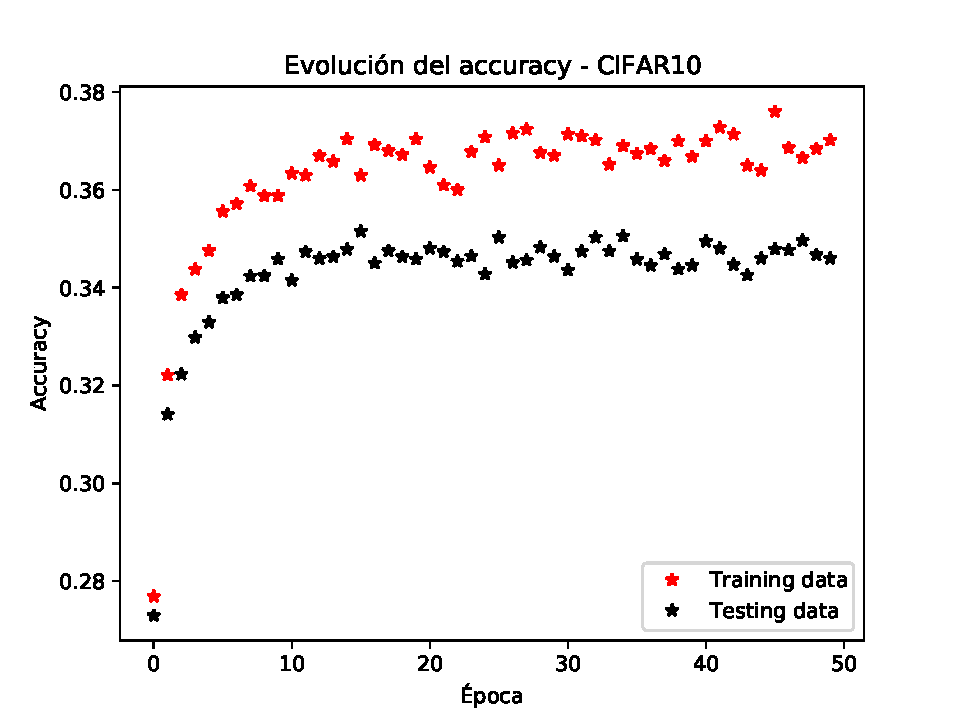
\includegraphics[width=\textwidth]{image/EJ4_Acc.pdf}
         \caption{Accuracy para el usando la función de costo CCE}
         \label{fig:acc6a}
     \end{subfigure}
     \hfill
     \begin{subfigure}[b]{0.45\textwidth}
         \centering
         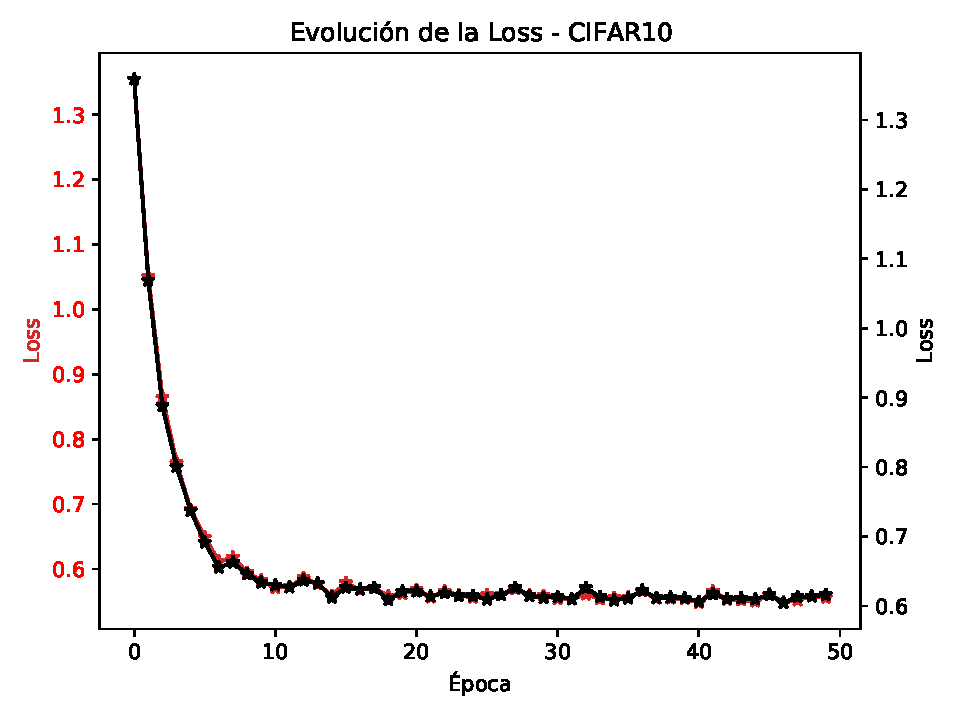
\includegraphics[width=\textwidth]{image/EJ4_Loss.pdf}
         \caption{Loss para el usando la función de costo CCE}
         \label{fig:loss6a}
     \end{subfigure}
        \caption{Resultados obtenidos del ejercicio 4}
        \label{fig:ej5_TP1}
\end{figure}
donde los parámetros del problema son:
\begin{verbatim}
nclases = 10  # neuronas capa de salida
nintermedia = 100  # neuronas capa intermedia
batch_size = 128  # tamaño del batch
n_epocas = 50  # cantidad de épocas para entrenar la red
learning_rate = 1e-3  # tasa de aprendizaje
reg_lambda = 1e-3  # factor de regularización
n_train_data = 5000  # cantidad de datos tomados para el entrenamiento
\end{verbatim}

La comparación solicitada en este punto es la misma que la del inciso 3 (ver figura \ref{fig:ej3})